%% =====================================================================
%% Manuscript for submission to Natural Hazards (Springer Nature)
%% Template: Springer Nature LaTeX template (sn-jnl.cls), sn-basic
%% (author-year) reference style, as used by Natural Hazards.
%%
%% Section order follows the author's structure:
%%  Abstract | Introduction | Literature survey | Problem statement and
%%  research gap | Novelty and proposed algorithm | Dataset and data
%%  preprocessing | Methodology | Evaluation metrics | Result evaluation
%%  | Conclusion and future work | References
%%
%% BEFORE SUBMISSION
%%  1. Search for \tofill -- every red placeholder must be replaced.
%%     Results, Abstract numbers and Conclusions MUST come from the
%%     experiments on the real Kerala data (not the synthetic test).
%%  2. Confirm no \tofill remains:  grep tofill main.tex
%% =====================================================================

\documentclass[pdflatex,sn-basic]{sn-jnl}

\usepackage{graphicx}%
\usepackage{multirow}%
\usepackage{amsmath,amssymb,amsfonts}%
\usepackage{amsthm}%
\usepackage{mathrsfs}%
\usepackage[title]{appendix}%
\usepackage{xcolor}%
\usepackage{textcomp}%
\usepackage{manyfoot}%
\usepackage{booktabs}%
\usepackage{algorithm}%
\usepackage{algorithmicx}%
\usepackage{algpseudocode}%
\usepackage{makecell}%
\usepackage{tikz}%
\usetikzlibrary{arrows.meta,positioning,shapes.geometric,calc}
\usepackage{lineno}%
\linenumbers

%% placeholder marker -- must not remain in the submitted file
\newcommand{\tofill}[1]{\textcolor{red}{[#1]}}

\theoremstyle{plain}%
\newtheorem{proposition}{Proposition}%
\theoremstyle{remark}%
\newtheorem{remark}{Remark}%
\theoremstyle{definition}%
\newtheorem{definition}{Definition}%

\raggedbottom

\begin{document}

\title[Calibration-guided reallocation of flood emergency resources]{Calibration-guided robust reallocation of emergency resources under evolving flood risk forecasts: a digital twin framework applied to the 2018 Kerala floods}

\author[1,2]{\fnm{Dannuri} \sur{Mounika}}\email{dmounikaresearch@gmail.com}
\author*[1]{\fnm{Johnson} \sur{Kolluri}}\email{johnson.kolluri@sru.edu.in}

\affil*[1]{\orgdiv{School of Computer Science \& Artificial Intelligence}, \orgname{SR University}, \orgaddress{\city{Warangal}, \postcode{506371}, \state{Telangana}, \country{India}}}
\affil[2]{\orgdiv{Department of CSE-AIML}, \orgname{TKR College of Engineering and Technology}, \orgaddress{\city{Hyderabad}, \postcode{500097}, \state{Telangana}, \country{India}}}

%% Natural Hazards: 150--250 words
\abstract{In the first days of a major flood, disaster management authorities must place scarce rescue teams, boats and medical units while risk forecasts keep changing and roads close to floodwater and landslides. Existing allocation models describe forecast uncertainty with hand-tuned budgets, so the protection a plan offers is not tied to how reliable the forecasts actually are. This study links the two. District-level conformal prediction sets from a flood risk model are converted, through an exposure and vulnerability model, into demand ranges that contain the true demand with a chosen probability $1-\alpha$. A robust allocation model then assigns resources, with travel times that grow with predicted inundation depth, routes closed by landslides removed, and a cost for moving teams. A trigger rule re-plans only when forecasts, risk classes or road conditions change enough to justify it. The framework is evaluated on a hindcast of the August 2018 Kerala floods across \tofill{N} units, with the August 2019 floods held out as an independent test, against static, proportional, stochastic, fixed-budget robust and learned allocation policies. \tofill{Main quantitative findings against the best baseline: unmet demand, response time, coverage, relocations.} \tofill{Result on the 2019 hold-out event and the stress scenarios.} The framework gives State and District Disaster Management Authorities one interpretable reliability setting and a stated reason for each redeployment.}

\keywords{Flood emergency response, Resource allocation, Kerala floods, Conformal prediction, Robust optimization, Digital twin}

\maketitle

%% =====================================================================
\section{Introduction}\label{sec:intro}

Floods are among the most damaging recurrent hazards in India, and their impacts concentrate in districts where exposure and vulnerability are high \citep{Saharia2025,Jain2025}. In the first days of a major flood, where scarce rescue resources are placed decides how many trapped and displaced people are reached in time. The August 2018 Kerala floods killed 433 people, affected 5.4 million and displaced 1.4 million, and water was released from 37 dams \citep{PDNA2018}. About 341 landslides occurred during the same event, many of them in the hill districts of Idukki and Wayanad, cutting the roads on which rescue teams depended \citep{PDNA2018}. The National Disaster Response Force (NDRF) made its largest deployment in a single state, sending 58 teams across ten severely affected districts \citep{NDRF2018}. The difficulty was not only the number of teams but where they were placed as the flood spread, as dam releases changed river levels and as roads became impassable.

Forecasting has advanced faster than the decisions that depend on it. Deep learning models now map flood susceptibility at regional scale \citep{Rachit2026}, coupled hydrologic--hydraulic systems forecast inundation depth with 48-hour lead times \citep{Rao2024}, and conformal methods are being extended to give reliable intervals for extreme events \citep{Pasche2026}. Yet a forecast helps responders only when it is turned into an allocation that still holds up if the forecast is wrong. Model reliability also changes over time: a model that performs well within its calibration period can lose accuracy in later periods \citep{Xiao2026}. Decision models therefore need to know how far each forecast can be trusted, and need to adapt as forecasts are updated.

The step from hazard to decision is where the hazard literature is thinnest. A recent systematic review of 80 studies on landslides affecting roads found that 90\% assessed susceptibility or hazard, but only 21\% completed the chain from hazard to consequence to risk, only 9\% modelled network connectivity and only 10\% quantified indirect losses \citep{Vega2026}. Studies that do model emergency logistics usually take forecasts as given, with uncertainty budgets chosen by the modeller \citep{Caunhye2012,Zhang2023}. The protection a plan offers is therefore not tied to the measured reliability of the forecasts that drive it, and re-planning at every period can move teams back and forth as forecasts fluctuate.

This study builds a decision framework for flood response that closes that link. It converts calibrated hazard forecasts into demand ranges with a stated reliability, allocates resources so that the plan holds across those ranges on a road network that degrades with flood depth and landslide blockage, and re-plans only when the situation has changed enough to justify moving teams. The framework is tested on the 2018 Kerala floods and, as an independent check, on the August 2019 Kerala floods.

The study addresses three research questions:
\begin{enumerate}
\item[RQ1.] Do demand ranges built from calibrated flood risk forecasts reduce worst-case unmet demand compared with fixed or hand-tuned ranges, at similar operational cost?
\item[RQ2.] Can a forecast-triggered re-planning rule match the coverage of re-planning at every period with fewer re-plans and team relocations?
\item[RQ3.] Does linking travel times to predicted inundation depth and observed landslide blockages reduce failed dispatches on the roads that actually closed?
\end{enumerate}

The contributions are as follows. (1) A procedure that converts district-level conformal prediction sets of flood risk classes into demand ranges with a coverage interpretation, so that a single setting $\alpha$ controls how cautious the plan is. (2) A robust allocation model with inundation-dependent travel times, landslide road closures and an explicit cost for relocating teams, with two supporting properties: its robust form is exact and linear, and calibrated forecasts give a probabilistic bound on unmet demand. (3) A forecast-triggered re-planning rule that gives authorities a stated reason for each redeployment. (4) A hindcast evaluation on the 2018 Kerala floods, with the 2019 floods held out, against five baselines, with ablations and stress scenarios, and recommendations for disaster management authorities.

Section~\ref{sec:lit} surveys the literature and Section~\ref{sec:gap} states the problem and the research gap. Section~\ref{sec:novelty} presents the novel components and the proposed algorithm. Section~\ref{sec:data} describes the study area, data and preprocessing, and Section~\ref{sec:method} the methodology. Section~\ref{sec:metrics} defines the evaluation metrics, Section~\ref{sec:results} reports and discusses the results, and Section~\ref{sec:conclusion} concludes.

%% =====================================================================
\section{Literature survey}\label{sec:lit}

\subsection{Flood risk forecasting and its reliability}

Flood risk models in India now operate at several scales. A district-level flood severity index combines hazard, exposure and vulnerability for national flood management \citep{Saharia2025}, and analysis of flood risk attributes has been used to identify where flood policy can improve \citep{Jain2025}. At regional scale, CNN--U-Net segmentation has produced rapid flood susceptibility maps for the Indian Himalayan region \citep{Rachit2026}, and integrated hydrologic--hydraulic models provide real-time inundation forecasts with 48-hour lead times in eastern India \citep{Rao2024}. For Kerala 2018, Sentinel-1 synthetic aperture radar (SAR) flood maps have been produced with about 94\% overall accuracy \citep{Tiwari2020}, and the geomorphic processes of the event have been linked to monsoon circulation and land use change \citep{Chothodi2024}. A common limitation is that model reliability is reported as an average accuracy, and that reliability can drift as conditions change between calibration and use \citep{Xiao2026}.

\subsection{Calibrated uncertainty for hazard forecasts}

Conformal prediction constructs prediction sets that contain the true outcome with probability at least $1-\alpha$ under exchangeability, without distributional assumptions \citep{Vovk2005,Angelopoulos2023}. \citet{Pasche2026} combined extreme value statistics with conformal prediction to obtain reliable intervals for rare, high-impact events such as floods. \citet{Johnstone2021} showed that conformal prediction regions can serve as robust-optimization uncertainty sets with finite-sample guarantees, illustrated on simulated examples. Their use for sizing the uncertainty in disaster response decisions has, to our knowledge, not been explored.

\subsection{Emergency resource allocation under uncertainty}

Optimization models for emergency logistics are reviewed by \citet{Caunhye2012}. Robust optimization protects a plan against every outcome in an uncertainty set \citep{BenTal2009,BertsimasSim2004}; \citet{BenTal2011} applied an affinely adjustable robust model to emergency logistics with time-varying demand, and \citet{Avishan2023} used adjustable robust optimization for relief distribution when damaged roads make travel times uncertain. For floods, \citet{Manopiniwes2021} formulated a multi-period location--routing model for temporary depots with multimodal transport. Rolling-horizon models re-solve as demand is revealed, for example in a hybrid robust--fuzzy model for earthquake relief \citep{Attar2026}, and \citet{Zhang2023} adjusted the uncertainty budget over a rolling horizon to reduce conservativeness as an epidemic evolved. Only about one in ten humanitarian logistics optimization studies involved practitioners, and model objectives often differed from practitioners' priorities \citep{RodriguezEspindola2023}, which argues for models whose settings authorities can interpret.

\subsection{Road network disruption by floods and landslides}

Floodwater slows and eventually stops road vehicles. \citet{Pregnolato2017} derived a depth--disruption function relating vehicle speed to standing water depth. \citet{He2026} combined flood hazard curves with vehicle fragility curves and found that flood exposure can restrict ambulance access to high-risk areas. Landslides add a second source of closure: \citet{Postance2017} assessed landslide disruptions on a national road network, \citet{Zhang2020} linked landslide likelihood to transport network vulnerability, and \citet{Zhang2021} quantified indirect economic losses of landslides along highways. Globally, road risk from landslides is projected to rise under climate change \citep{Duan2025}. These studies quantify disruption but rarely feed it into the allocation of response resources \citep{Vega2026}.

\subsection{Digital twins and learning-based dispatch}

Digital twins couple live observations with simulation models of a hazard and the systems it affects. \citet{Liu2026} combined a digital twin, an optimization model and a deep Q-network for urban emergency distribution during the Zhengzhou ``7$\cdot$20'' rainstorm. Reviews of digital twin cities for flood evacuation \citep{Prihatmanto2025}, of digital twins in safety and emergency management \citep{Zio2024}, and of digital twin-based decision support for natural disasters \citep{Inyang2025} identify data integration, model accuracy and limited treatment of uncertainty as open problems. Reinforcement learning has been used to dispatch rescue teams during floods \citep{Yan2020} and to assign rescue helicopters \citep{Shen2023}. These methods respond quickly once trained, but offer no coverage guarantee and are hard for authorities to audit.

\subsection{Comparison with closely related studies}

Table~\ref{tab:gap} compares this study with the closest work.

\begin{table}[h]
\caption{Comparison with closely related studies}\label{tab:gap}
\footnotesize
\setlength{\tabcolsep}{3pt}
\begin{tabular*}{\textwidth}{@{\extracolsep\fill}lccccccc}
\toprule
Study & \makecell{Dynamic\\re-planning} & \makecell{Sets from\\calibrated\\forecasts} & \makecell{Coverage\\guarantee} & \makecell{Inundation-\\dependent\\travel} & \makecell{Landslide\\road\\closures} & \makecell{Relocation\\cost or\\trigger} & \makecell{Real\\flood\\case} \\
\midrule
\citet{Liu2026} & Yes & No & No & Partly & No & No & Yes \\
\citet{Attar2026} & Yes & No & No & No & No & No & No \\
\citet{Zhang2023} & Yes & No & No & No & No & No & No \\
\citet{Yan2020} & Yes & No & No & Yes & No & No & Yes \\
\citet{Avishan2023} & Yes & No & No & No & Partly & No & No \\
\citet{Manopiniwes2021} & Yes & No & No & No & No & No & Yes \\
\citet{Johnstone2021} & No & Yes & Yes & No & No & No & No \\
This study & Yes & Yes & Yes & Yes & Yes & Yes & Yes \\
\botrule
\end{tabular*}
\end{table}

%% =====================================================================
\section{Problem statement and research gap}\label{sec:gap}

\subsection{Problem statement}

A state disaster management authority holds a fixed stock of rescue teams, boats and medical units at staging bases. Over a flood event divided into decision periods $t = 1, \dots, T$, it must decide how many units of each resource to send from each base to each affected unit (district or taluk). At each period it receives updated forecasts of the flood risk class of every unit and of inundation depth along roads, together with reports of roads closed by landslides. The true number of people needing assistance in each unit is unknown when the decision is made. The authority wants to (i) minimize unmet demand, weighted towards vulnerable units, including in the worst case across plausible forecast errors; (ii) reach people quickly; (iii) avoid sending resources along roads that are flooded beyond their capability or blocked; and (iv) avoid moving teams back and forth when forecasts change only slightly.

\subsection{Research gap}

The literature in Section~\ref{sec:lit} leaves four gaps.
\begin{enumerate}
\item[G1.] \textbf{Uncertainty in allocation is not tied to forecast reliability.} Robust and rolling-horizon allocation models size their uncertainty sets by hand or heuristically \citep{BenTal2011,Zhang2023,Attar2026}, so a plan's protection has no stated link to how often the forecasts that drive it are wrong.
\item[G2.] \textbf{Hazard studies rarely reach the decision stage.} Most studies stop at susceptibility or hazard; few model network consequences or indirect losses, and fewer still turn them into response decisions \citep{Vega2026}.
\item[G3.] \textbf{Road disruption is treated separately from allocation.} Depth--disruption and landslide--network studies quantify which roads fail \citep{Pregnolato2017,Postance2017,He2026}, but allocation models rarely use predicted depth or landslide blockage to decide which resource type can reach a unit.
\item[G4.] \textbf{Re-planning has no stated rule.} Rolling-horizon and learned dispatch methods re-plan every period \citep{Attar2026,Yan2020,Liu2026}, which can move teams back and forth and gives authorities no reason for each redeployment.
\end{enumerate}
RQ1 addresses G1 and G2, RQ2 addresses G4 and RQ3 addresses G3.

%% =====================================================================
\section{Novelty and proposed algorithm}\label{sec:novelty}

\subsection{Novel elements}

The framework introduces four elements that, to our knowledge, have not been combined for flood emergency response. (N1) \emph{Calibrated demand ranges}: conformal prediction sets of flood risk classes are mapped through exposure and vulnerability into demand ranges with coverage at least $1-\alpha$ (Sect.~\ref{sec:bridge}). (N2) \emph{Data-driven uncertainty budget}: the number of units allowed to reach their upper demand together is set from calibration data rather than by hand (Definition~\ref{def:set}). (N3) \emph{Hazard-aware reachability}: travel times grow with predicted inundation depth, and routes deeper than a resource can cross or blocked by mapped landslides are excluded (Eq.~\ref{eq:travel}). (N4) \emph{Forecast-triggered re-planning}: the plan is revised only on a material forecast shift, a risk-class escalation or a route failure (Sect.~\ref{sec:trigger}). We call the combined method calibration-guided robust reallocation (CGRR). Novelty is claimed for the combination and its application to flood response; conformal sets for robust optimization exist in general \citep{Johnstone2021}.

\subsection{Framework overview}

The framework repeats four stages at each decision period (Fig.~\ref{fig:framework}). (i) The forecasting layer issues risk class probabilities, conformal prediction sets and predicted inundation depths, and the road layer reports landslide closures. (ii) An exposure model converts the conformal sets into unit demand ranges and a budgeted uncertainty set. (iii) A trigger rule decides whether the current plan should be revised. (iv) If so, a robust allocation model computes a new plan, which the digital twin then executes against the realized flood.

\begin{figure}[h]
\centering
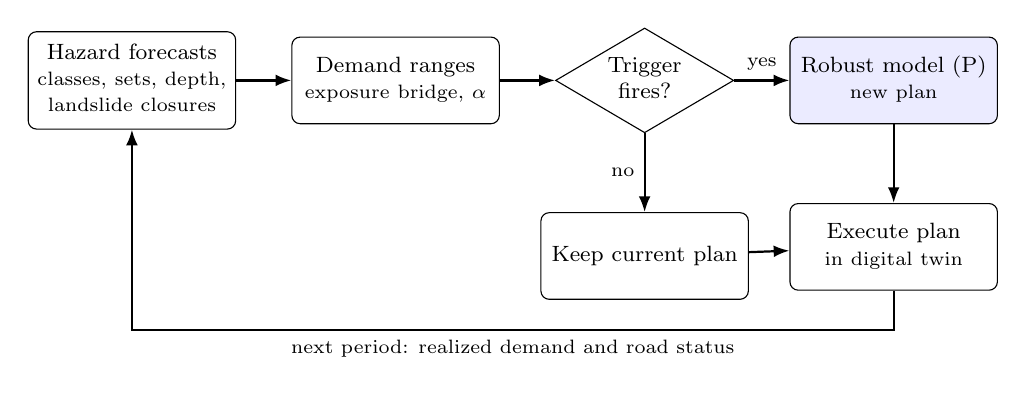
\begin{tikzpicture}[
  node distance=6mm and 7mm,
  box/.style={draw, rounded corners=3pt, align=center, minimum height=11mm, text width=24mm, font=\footnotesize},
  dec/.style={draw, diamond, aspect=1.7, align=center, inner sep=1pt, font=\footnotesize},
  arr/.style={-{Latex[length=2mm]}, thick}]
\node[box] (fc) {\begin{tabular}{@{}c@{}}\footnotesize Hazard forecasts\\\fontsize{7pt}{8pt}\selectfont classes, sets, depth,\\\fontsize{7pt}{8pt}\selectfont landslide closures\end{tabular}};
\node[box, right=of fc] (us) {\begin{tabular}{@{}c@{}}\footnotesize Demand ranges\\\fontsize{7pt}{8pt}\selectfont exposure bridge, $\alpha$\end{tabular}};
\node[dec, right=of us] (tr) {\begin{tabular}{@{}c@{}}\footnotesize Trigger\\\footnotesize fires?\end{tabular}};
\node[box, right=of tr, fill=blue!8] (rm) {\begin{tabular}{@{}c@{}}\footnotesize Robust model (P)\\\fontsize{7pt}{8pt}\selectfont new plan\end{tabular}};
\node[box, below=10mm of tr] (kp) {\footnotesize Keep current plan};
\node[box, below=10mm of rm] (ex) {\begin{tabular}{@{}c@{}}\footnotesize Execute plan\\\fontsize{7pt}{8pt}\selectfont in digital twin\end{tabular}};
\draw[arr] (fc) -- (us);
\draw[arr] (us) -- (tr);
\draw[arr] (tr) -- node[above, font=\fontsize{7pt}{8pt}\selectfont]{yes} (rm);
\draw[arr] (tr) -- node[left, font=\fontsize{7pt}{8pt}\selectfont]{no} (kp);
\draw[arr] (rm) -- (ex);
\draw[arr] (kp) -- (ex);
\draw[arr] (ex.south) -- ++(0,-5mm) -| node[pos=0.25, below, font=\fontsize{7pt}{8pt}\selectfont]{next period: realized demand and road status} (fc.south);
\end{tikzpicture}
\caption{The framework loop at each decision period. The robust model is solved only when the trigger fires; otherwise the current plan stays in force}\label{fig:framework}
\end{figure}

\subsection{Proposed algorithm}

Algorithm~\ref{alg:trigger} gives the complete procedure for one event. Equations are defined in Section~\ref{sec:method}.

\begin{algorithm}[h]
\caption{Calibration-guided robust reallocation (CGRR) over one flood event}\label{alg:trigger}
\begin{algorithmic}[1]
\Require calibration data; level $\alpha$; trigger threshold $\eta$; stocks $S_{r,j}$; road network
\State fit split conformal predictor on calibration periods; set $\Gamma$ from calibration data (Def.~\ref{def:set})
\State $\bar x \gets$ undefined
\For{$t = 1, \dots, T$}
  \State obtain forecasts $(\hat p_t, C_t, \hat h_t)$ and landslide closures $L_t$
  \State compute $d^{L}_t, \hat d_t, d^{U}_t$ by \eqref{eq:bridge} and $\mathcal{U}_t(\alpha)$ by \eqref{eq:set}
  \State compute $\tau_{j,i,t}$ and passability by \eqref{eq:travel}, removing routes in $L_t$
  \If{$\bar x$ undefined \textbf{or} $\Delta_t > \eta$ \textbf{or} an upper class of $C_t$ rises \textbf{or} a used route is impassable}
    \State solve (P) with reference plan $\bar x$; set $\bar x \gets x^{\ast}_t$, $\tau \gets t$
  \EndIf
  \State execute $\bar x$ in the digital twin; record realized demand, service and travel times
\EndFor
\end{algorithmic}
\end{algorithm}

%% =====================================================================
\section{Dataset and data preprocessing}\label{sec:data}

\subsection{Study area: the August 2018 Kerala floods}

Kerala, on India's south-west coast, experienced its most severe flooding in decades in August 2018. Intense rainfall from the night of 8--9 August, together with water released from 37 dams, flooded river basins across all 14 districts and triggered about 341 landslides \citep{PDNA2018,NDRF2018}. NDRF deployed 58 teams, concentrated in Pathanamthitta, Idukki, Alappuzha, Wayanad, Kottayam, Ernakulam, Thrissur, Kozhikode, Thiruvananthapuram and Malappuram districts; its teams rescued 535 people and evacuated 24,690 \citep{NDRF2018}. In total, 1.4 million people were displaced and 1,259 of the state's 1,664 villages were affected \citep{PDNA2018}.

The event suits this study for three reasons. Demand shifted across districts within days as dam releases moved floodwater downstream. Rescue resources were of several types, with different abilities to cross deep water. And flood extent, landslide, population and road data are publicly available, which allows a hindcast. The August 2019 Kerala floods, which again combined riverine flooding with landslides in the hill districts \tofill{citation}, serve as an independent test event that is never used for calibration or tuning.

\begin{figure}[h]
\centering
\fbox{\parbox[c][4cm][c]{0.8\textwidth}{\centering\tofill{Figure 2: map of Kerala showing the decision units, observed peak flood extent (Sentinel-1), mapped landslides on roads, staging bases and the main road network.}}}
\caption{Study area \tofill{caption details, no final full stop}}\label{fig:map}
\end{figure}

\subsection{Data sources}

The decision units are \tofill{taluks or the 14 districts}, $|I| = \tofill{N}$, over \tofill{8--25 August 2018} in 6-hour decision periods. Resources are rescue teams, boats and medical units staged at \tofill{bases from deployment records}. Table~\ref{tab:data} lists the data.

\begin{table}[h]
\caption{Data used in the study}\label{tab:data}
\footnotesize
\begin{tabular*}{\textwidth}{@{\extracolsep\fill}p{3.4cm}p{3.6cm}p{4.4cm}}
\toprule
Data & Use in the model & Source \\
\midrule
Risk class probabilities and conformal sets & Demand ranges (Sect.~\ref{sec:bridge}) & Flood risk model with split conformal prediction, re-run for each event \\
Predicted inundation depth & Travel time and passability & Flood digital twin inundation forecast \\
Observed flood extent & Realized demand and flooded roads & Sentinel-1 SAR (Copernicus), via Google Earth Engine \citep{Tiwari2020} \\
Landslide locations & Road closures & 2018: inventory of 4,728 landslides \citep{Hao2020}; 2019: \tofill{source} \\
Relief-camp occupancy & Independent check of realized demand & District-wise camps and inmates, 2018 \citep{GoK2018Memo}; 2019: \tofill{source} \\
Population & Exposed population $P_i$ & Census of India 2011 (projected) or WorldPop \\
Social vulnerability & Weights $w_i$ and multipliers $v_i$ & Index from Census variables; District Flood Severity Index \citep{Saharia2025} \\
Road network & Normal travel times $\tau^0_{j,i}$ & OpenStreetMap \\
Resources and bases & $S_{r,j}$, $\kappa_r$ & NDRF situation reports \citep{NDRF2018,NDRF2018b,NDRF2019} \\
Damage fraction per class & $\delta_k$ & Historical flood damage and relief-camp records; IFI-Impacts database \citep{Saharia2025} \\
\botrule
\end{tabular*}
\end{table}

\subsection{Data preprocessing}

All methods compared in Section~\ref{sec:results} use the same preprocessed inputs, so that differences in results come from the allocation method alone.

\subsubsection{Flood extent}
 Sentinel-1 ground-range-detected scenes in vertical--vertical (VV) polarization over Kerala are speckle-filtered, terrain-corrected and thresholded to water/non-water with an automatic threshold, following \citet{Tiwari2020}. Permanent water bodies are masked. Each scene is assigned to the decision period in which it was acquired; between acquisitions the flood extent is held at the last observation. \tofill{Scene dates and the number of periods covered by each scene.}

\subsubsection{Exposed population}
 Gridded population is overlaid on the flood extent for each period to give the exposed population $P_{i,t}$ of each unit; the maximum over the event gives $P_i$.

\subsubsection{Road network and travel times}
 The OpenStreetMap road network is clipped to Kerala and converted to a routable graph. Normal travel times $\tau^0_{j,i}$ are shortest-path times from each base to the population-weighted centroid of each unit, using road-class speeds. Predicted depth on each route $\hat h_{j,i,t}$ is the maximum forecast inundation depth sampled along the route.

\subsubsection{Landslide road closures}
 Mapped landslides within \tofill{50 m} of a road segment close that segment from the date of the landslide until \tofill{the reported reopening date, or the end of the event if unknown}. Routes that cross a closed segment are recomputed or marked impassable.

\subsubsection{Vulnerability}
 Census variables \tofill{list} are normalized and combined into an index; $w_i$ and $v_i$ are its rescaled values.

\subsubsection{Realized demand and its check}
 Realized demand in each unit and period is the exposed population multiplied by the damage fraction of its observed risk class. Because the forecast-side demand uses the same damage fractions, realized demand is also compared with district-wise relief-camp occupancy, an observation that does not depend on the model. \tofill{Rank correlation between modelled and observed district demand.}

\subsubsection{Calibration and test split}
 The conformal predictor is calibrated on \tofill{monsoon periods before August 2018}. The 2018 event is the main test; the 2019 event is a held-out test that is never used for calibration or for tuning $\alpha$, $\eta$, $\beta$, $\lambda$ or $\mu$. Tuning uses \tofill{a validation period}.

%% =====================================================================
\section{Methodology}\label{sec:method}

\subsection{From conformal prediction sets to demand ranges}\label{sec:bridge}

For unit $i$ at time $t$, the forecasting model gives class probabilities $\hat p_{i,t,k}$ over risk classes $k \in K = \{\text{low}, \text{medium}, \text{high}, \text{severe}\}$ and a conformal prediction set $C_{i,t} \subseteq K$ with coverage at least $1-\alpha$. Each class has a damage fraction $\delta_k$, the share of exposed people needing assistance. With exposed population $P_i$ and vulnerability multiplier $v_i$,
\begin{equation}
d^{L}_{i,t} = v_i P_i \min_{k \in C_{i,t}} \delta_k, \qquad
d^{U}_{i,t} = v_i P_i \max_{k \in C_{i,t}} \delta_k, \qquad
\hat d_{i,t} = v_i P_i \sum_{k \in K} \hat p_{i,t,k}\, \delta_k .
\label{eq:bridge}
\end{equation}

\begin{definition}[Calibrated budgeted uncertainty set]\label{def:set}
For a budget $\Gamma_t \in \{0, 1, \dots, |I|\}$,
\begin{equation}
\mathcal{U}_t(\alpha) = \Big\{ d : d_{i,t} = \hat d_{i,t} + z_i\,(d^{U}_{i,t} - \hat d_{i,t}),\; 0 \le z_i \le 1,\; \sum_{i} z_i \le \Gamma_t \Big\}.
\label{eq:set}
\end{equation}
\end{definition}

$\Gamma_t$ limits how many units can reach their upper bound together. It is set from the calibration data as the 95th percentile, over calibration periods, of the number of units whose realized damage fraction exceeded the point estimate. Smaller $\alpha$ widens the ranges and makes plans more cautious.

\subsection{Robust reallocation model}

Let $I$ be the units, $J$ the staging bases and $R$ the resource types. Resource $r$ serves $\kappa_r$ people per period, base $j$ holds $S_{r,j}$ units of it, and $w_i$ is the vulnerability weight of unit $i$. The normal travel time is $\tau^0_{j,i}$, the predicted maximum inundation depth on the route is $\hat h_{j,i,t}$, and resource $r$ can cross water up to depth $h^{\max}_r$. The decision $x_{r,j,i,t} \in \mathbb{Z}_{+}$ is the number of units of $r$ sent from $j$ to $i$; $\bar x_{t-1}$ is the plan in force.

Travel times grow with predicted inundation, a linear approximation of the depth--disruption relation of \citet{Pregnolato2017}. Routes that are too deep, too slow or blocked by a landslide ($L_t$ is the set of blocked base--unit routes) are excluded:
\begin{equation}
\tau_{j,i,t} = \tau^{0}_{j,i}\,\big(1 + \beta\, \hat h_{j,i,t}\big), \qquad
x_{r,j,i,t} = 0 \;\; \text{if} \;\; \hat h_{j,i,t} > h^{\max}_{r},\; \tau_{j,i,t} > \tau^{\max} \;\text{or}\; (j,i) \in L_t .
\label{eq:travel}
\end{equation}
Boats are given a large $h^{\max}_r$ but cannot use routes blocked by landslides on hill roads. With coverage $\mathrm{cov}_{i,t} = \sum_{r}\sum_{j} \kappa_r x_{r,j,i,t}$, model (P) is
\begin{align}
\min \;& \sum_{i} w_i u_{i,t} + \Gamma_t\theta_t + \sum_{i}\pi_{i,t} + \lambda \sum_{r,j,i}\tau_{j,i,t}\,x_{r,j,i,t} \nonumber\\
&\quad + \mu \sum_{r,j,i}\big(y^{+}_{r,j,i,t} + y^{-}_{r,j,i,t}\big) + M \sum_{i \in I^{\mathrm{v}}} w_i e_{i,t} \label{eq:obj}\\
\text{s.t.}\;& u_{i,t} \ge \hat d_{i,t} - \mathrm{cov}_{i,t}, \quad a_{i,t} \ge d^{U}_{i,t} - \mathrm{cov}_{i,t} && \forall i, \label{eq:short}\\
& \theta_t + \pi_{i,t} \ge w_i\,(a_{i,t} - u_{i,t}) && \forall i, \label{eq:dual}\\
& \textstyle\sum_{i} x_{r,j,i,t} \le S_{r,j} && \forall r, j, \label{eq:supply}\\
& \mathrm{cov}_{i,t} + e_{i,t} \ge \rho\, d^{L}_{i,t} && \forall i \in I^{\mathrm{v}}, \label{eq:equity}\\
& x_{r,j,i,t} - \bar x_{r,j,i,t-1} = y^{+}_{r,j,i,t} - y^{-}_{r,j,i,t} && \forall r, j, i, \label{eq:reloc}\\
& x \in \mathbb{Z}_{+},\; u, a, y^{\pm}, e, \theta, \pi \ge 0. \nonumber
\end{align}
Here $u$ is nominal unmet demand, $a$ is unmet demand at the upper bound, $\theta$ and $\pi$ are dual variables of the robust counterpart, and $\lambda$ and $\mu$ weight response time and relocation. Constraint~\eqref{eq:equity} is an equity floor for the most vulnerable units $I^{\mathrm v}$; it is soft, with penalty $M$, so the model stays feasible when flooded or blocked roads make a vulnerable unit unreachable. Model (P) is solved one period at a time; the relocation term links consecutive periods.

\subsection{Properties of the model}

\begin{proposition}\label{prop:exact}
For fixed coverage and integer $\Gamma_t$, the minimum of $\sum_i w_i u_{i,t} + \Gamma_t\theta_t + \sum_i \pi_{i,t}$ subject to \eqref{eq:short}--\eqref{eq:dual} and non-negativity equals the worst-case weighted unmet demand over $\mathcal{U}_t(\alpha)$.
\end{proposition}

\begin{proof}
See Appendix~\ref{secA1}.
\end{proof}

In plain terms, Proposition~\ref{prop:exact} means the linear model (P) protects against the worst combination of up to $\Gamma_t$ units reaching their upper demand, with no approximation, so standard solvers can be used.

\begin{proposition}\label{prop:bound}
Assume (A1) calibration and test units are exchangeable, so that $P(k^{\star}_i \in C_i) \ge 1-\alpha$ for the true class $k^{\star}_i$, and (A2) realized demand satisfies $d_i \le v_i P_i \delta_{k^{\star}_i}$. Then for any plan $x$, the realized shortfall $s_i$ of each unit satisfies $P\big(s_i \le a_i(x)\big) \ge 1-\alpha$, and
\begin{equation}
\mathbb{E}\Big[\sum_{i} w_i \big(s_i - a_i(x)\big)^{+}\Big] \;\le\; \alpha \sum_{i} w_i\, v_i P_i \big(\delta_{\max} - \delta_{\min}\big),
\label{eq:bound}
\end{equation}
where $\delta_{\max}$ and $\delta_{\min}$ are the largest and smallest damage fractions.
\end{proposition}

\begin{proof}
If $k^{\star}_i \in C_i$, then $d_i \le v_i P_i \delta_{k^\star_i} \le d^U_i$, so $s_i = (d_i - \mathrm{cov}_i)^+ \le (d^U_i - \mathrm{cov}_i)^+ = a_i(x)$. Otherwise $(s_i - a_i(x))^+ \le (d_i - d^U_i)^+ \le v_i P_i(\delta_{\max} - \delta_{\min})$, a constant. Hence $(s_i - a_i(x))^+ \le \mathbf{1}\{k^{\star}_i \notin C_i\}\, v_i P_i(\delta_{\max} - \delta_{\min})$, and the event $k^{\star}_i \notin C_i$ has probability at most $\alpha$ by (A1). Taking expectations and summing gives \eqref{eq:bound}. By linearity, the expected number of units whose shortfall exceeds $a_i(x)$ is at most $\alpha |I|$.
\end{proof}

\begin{remark}
Split conformal prediction guarantees marginal coverage under exchangeability. Flood periods are serially dependent, so (A1) may hold only approximately; Section~\ref{sec:results} therefore reports the empirical coverage on both test events, and stress scenario S3 measures what happens when coverage falls below its target. Class-conditional (Mondrian) conformal prediction can be used if guarantees are needed per risk class.
\end{remark}

\subsection{Forecast-triggered reallocation}\label{sec:trigger}

Re-solving (P) at every period can move teams back and forth as forecasts fluctuate. The plan in force since time $\tau$ is therefore revised only if at least one of three conditions holds. (1) Forecast shift: the weighted change in point demand, relative to the larger of the reference demand and the total response capacity per period $C = \sum_{r,j}\kappa_r S_{r,j}$, exceeds a threshold $\eta$,
\begin{equation}
\Delta_t = \frac{\sum_i w_i\,\lvert \hat d_{i,t} - \hat d_{i,\tau} \rvert}{\max\big(\sum_i w_i\, \hat d_{i,\tau},\; C\big)} > \eta .
\label{eq:trigger}
\end{equation}
The capacity floor stops near-zero demand early and late in the event from triggering re-planning. (2) Risk-class escalation: the upper class of $C_{i,t}$ rises for any unit. (3) Route failure: a route used by the current plan becomes impassable through flooding or a landslide. The rule plays the same role as tiered warning levels in operational early warning, where action is taken only when a defined level is crossed \citep{Metodiev2026}; here every redeployment comes with the condition that caused it.

\subsection{Use of AI tools}

\tofill{Springer Nature requires any use of large language models or other AI tools, beyond AI-assisted copy editing, to be described here: name the tool, what it was used for (e.g.\ code generation, drafting) and how outputs were checked. If none was used beyond copy editing, delete this subsection.}

\subsection{Hindcast simulator}

The digital twin replays each event period by period. Plans are made only from forecasts available at decision time and are then scored against realized demand and realized road closures; no method sees realized values when planning. Uncertainty in the damage fractions is represented by drawing $\delta_k$ for each run from \tofill{a distribution fitted to historical records, e.g.\ a Beta distribution per class}; each configuration is run \tofill{200} times, a number justified by the convergence of the coefficient of variation of the main metrics. Optimization models are solved with HiGHS through PuLP \tofill{or Gurobi; hardware}.

\subsection{Baselines and ablations}

Table~\ref{tab:baselines} lists the compared methods. All use the same inputs, decision periods and road closures. B5 is trained on \tofill{training events} and never on either test event. Ablation A1 replaces the conformal sets with fixed-width ($\pm 30\%$) ranges; A2a re-plans every period and A2b never re-plans; A3 plans with normal travel times and ignores landslide closures until a dispatch fails.

\begin{table}[h]
\caption{Compared methods}\label{tab:baselines}
\footnotesize
\begin{tabular*}{\textwidth}{@{\extracolsep\fill}llll}
\toprule
Code & Method & Uncertainty handling & Re-planning \\
\midrule
B1 & Static deterministic allocation & Point forecast & Once \\
B2 & Proportional-to-risk heuristic & None & Every period \\
B3 & Two-stage stochastic programming & Sampled scenarios & Every period \\
B4 & Rolling budgeted robust optimization & Hand-tuned fixed budget & Every period \\
B5 & Learned score-based dispatcher & Learned in simulator & Every period \\
CGRR & Proposed (Algorithm~\ref{alg:trigger}) & Conformal ranges & Triggered \\
\botrule
\end{tabular*}
\end{table}

\subsection{Sensitivity and stress scenarios}

We vary $\alpha \in \{0.05, 0.10, 0.20, 0.30\}$ and $\eta \in \{0, 0.05, 0.10, 0.20, 0.30\}$, and test three stress scenarios: S1, realized demand 30\% higher than the exposure model implies; S2, 25\% fewer resources; S3, forecast errors doubled at test time without recalibration, so that assumption A1 fails.

%% =====================================================================
\section{Evaluation metrics}\label{sec:metrics}

Let $s_{i,t} = (d_{i,t} - \mathrm{cov}_{i,t})^{+}$ be the realized shortfall of unit $i$ in period $t$, $D = \sum_{i,t} d_{i,t}$ the total realized demand and $\mathrm{RT}_{i,t}$ the time to the first passable resource arrival, capped at $\tau^{\max}$ for unserved demand. All metrics are computed on realized, not forecast, demand.

\subsection{Service metrics}

\begin{align}
\text{Total weighted unmet demand:}\quad & \mathrm{TWU} = \textstyle\sum_{i,t} w_i\, s_{i,t}, \label{eq:twu}\\
\text{Worst-unit weighted unmet demand:}\quad & \mathrm{WWU} = \textstyle\max_i \sum_{t} w_i\, s_{i,t}, \label{eq:wwu}\\
\text{Population coverage:}\quad & \mathrm{COV} = 1 - \textstyle\sum_{i,t} s_{i,t} / D, \label{eq:cov}\\
\text{Mean response time:}\quad & \overline{\mathrm{RT}} = \textstyle\sum_{i,t} d_{i,t}\, \mathrm{RT}_{i,t} / D, \label{eq:rt}
\end{align}
with the demand-weighted 95th percentile $\mathrm{RT}_{95}$ and the share of demand reached within 6 h reported alongside \eqref{eq:rt}. Missed high-risk unit-periods count the $(i,t)$ whose true class is severe and where $s_{i,t} > 0.5\, d_{i,t}$.

\subsection{Operational metrics}
 Team relocations $\mathrm{REL} = \sum_t \sum_{r,j,i} y^{+}_{r,j,i,t}$ over the event; the number of re-plans; failed dispatches, i.e.\ resources sent on a route that was impassable at the time of travel because of flooding or a landslide; and computation time per re-plan.

\subsection{Reliability metrics}
 Empirical coverage of the conformal sets, $\frac{1}{|I|T}\sum_{i,t}\mathbf{1}\{k^\star_{i,t} \in C_{i,t}\}$, compared with the target $1-\alpha$; mean set size; and the exceedance rate $\frac{1}{|I|T}\sum_{i,t}\mathbf{1}\{s_{i,t} > a_{i,t}\}$, compared with the bound $\alpha$ of Proposition~\ref{prop:bound}.

\subsection{Statistical testing}
 For each metric, CGRR is compared with each baseline across the paired simulation runs with the Wilcoxon signed-rank test, with Holm correction for multiple comparisons. Results are reported as medians with interquartile ranges and effect sizes, not as single best runs.

%% =====================================================================
\section{Result evaluation}\label{sec:results}
%% Write each subsection only after the real-data experiments.
%% Open with the finding and its number; use cautious wording.

\subsection{Forecast calibration on the test events}

\tofill{Empirical conformal coverage on the 2018 and 2019 events at $\alpha = 0.10$ (target 0.90), mean set size, and the observed exceedance rate compared with the bound of Proposition~\ref{prop:bound}. Rank correlation between modelled demand and relief-camp occupancy.}

\subsection{Comparison with baselines}

\tofill{Lead sentence with the main finding and its number.}

\begin{table}[h]
\caption{Performance on the 2018 Kerala hindcast: median over \tofill{200} runs, interquartile range in brackets. Bold: best; $^{\ast}$: CGRR differs significantly from the method (Wilcoxon, Holm-corrected $p<0.05$)}\label{tab:main}
\footnotesize
\begin{tabular*}{\textwidth}{@{\extracolsep\fill}lccccccc}
\toprule
Method & \makecell{Worst-unit\\weighted\\unmet} & \makecell{Total\\unmet\\(people)} & \makecell{Mean\\response\\(h)} & \makecell{P95\\response\\(h)} & \makecell{Coverage\\(\%)} & \makecell{Missed\\high-risk} & \makecell{Reloca-\\tions} \\
\midrule
B1 Static & \tofill{} & \tofill{} & \tofill{} & \tofill{} & \tofill{} & \tofill{} & \tofill{} \\
B2 Proportional & \tofill{} & \tofill{} & \tofill{} & \tofill{} & \tofill{} & \tofill{} & \tofill{} \\
B3 Stochastic & \tofill{} & \tofill{} & \tofill{} & \tofill{} & \tofill{} & \tofill{} & \tofill{} \\
B4 Fixed robust & \tofill{} & \tofill{} & \tofill{} & \tofill{} & \tofill{} & \tofill{} & \tofill{} \\
B5 Learned & \tofill{} & \tofill{} & \tofill{} & \tofill{} & \tofill{} & \tofill{} & \tofill{} \\
CGRR & \tofill{} & \tofill{} & \tofill{} & \tofill{} & \tofill{} & \tofill{} & \tofill{} \\
\botrule
\end{tabular*}
\end{table}

\subsection{Independent test: the 2019 Kerala floods}

\tofill{Same table for 2019, or a compact version. State whether the ranking of methods holds on the held-out event.}

\subsection{RQ1: value of calibrated demand ranges}

\tofill{CGRR versus ablation A1 and baseline B4: change in worst-unit unmet demand and cost; coverage--cost curve across $\alpha$ (Figure).}

\subsection{RQ2: triggered versus every-period re-planning}

\tofill{CGRR versus A2a and A2b: coverage, relocations and number of re-plans; trigger firings plotted against forecast shift, dam-release dates and landslide dates (Figure).}

\subsection{RQ3: inundation- and landslide-aware routing}

\tofill{CGRR versus A3: failed dispatches, split by flooding and landslide causes, and the resulting change in unmet demand and response time, especially in Idukki and Wayanad.}

\subsection{Sensitivity and stress scenarios}

\begin{table}[h]
\caption{Change of CGRR relative to the best baseline under each stress scenario}\label{tab:stress}
\footnotesize
\begin{tabular*}{\textwidth}{@{\extracolsep\fill}lccc}
\toprule
Scenario & \makecell{Unmet demand\\change (\%)} & \makecell{P95 response\\change (\%)} & \makecell{Coverage\\change (pp)} \\
\midrule
S1 Severe flood (+30\% demand) & \tofill{} & \tofill{} & \tofill{} \\
S2 Resource shortage ($-$25\%) & \tofill{} & \tofill{} & \tofill{} \\
S3 Forecast degradation & \tofill{} & \tofill{} & \tofill{} \\
\botrule
\end{tabular*}
\end{table}

\tofill{Paragraph on the $\eta$ sensitivity.}

\subsection{Discussion}

\subsubsection{Implications for disaster management authorities}
 The framework replaces a hand-tuned uncertainty budget with one setting, $\alpha$, that authorities can read as a reliability target: plan so that, for at least $(1-\alpha)$ of units, demand will not exceed what was prepared for. The trigger rule gives the Kerala State Disaster Management Authority, District Disaster Management Authorities and NDRF a stated reason for each redeployment, which a learned dispatcher cannot easily provide; such interpretability addresses the limited practitioner uptake of humanitarian optimization models \citep{RodriguezEspindola2023}. Because routes depend on predicted inundation and mapped landslides, the plan avoids sending road-based teams along roads the forecast already expects to flood or that are blocked, and sends boats or alternative routes instead. \tofill{Where the method helped most in 2018, for example units downstream of dam releases or hill districts cut off by landslides, and where it did not; compare candidly with the strongest baseline.}

\subsubsection{Relation to the forecasting chain}
 The value of the allocation depends on forecast calibration. Model reliability can shift between periods \citep{Xiao2026}, so the calibration set for the conformal layer should be refreshed from recent events. Scenario S3 shows how the plan degrades when coverage is lower than promised. Because the severe class is rare, extreme conformal methods \citep{Pasche2026} may give tighter guarantees where they matter most.

\subsubsection{Limitations}
 Demand is derived from exposure and damage fractions rather than observed rescue requests; relief-camp occupancy is used as an independent check but records people who reached camps, not those still waiting for rescue. The damage fractions carry their own uncertainty, which is propagated through the simulation runs. Landslide closure durations are approximate where reopening dates are not recorded. Proposition~\ref{prop:bound} relies on exchangeability and marginal coverage, which serially dependent flood data satisfy only approximately. The model does not represent crew fatigue, communication failures or coordination between agencies, and is solved one period at a time without multi-period look-ahead. Solve times grow with the number of units and resource types, so finer spatial units may need decomposition or heuristics.

%% =====================================================================
\section{Conclusion and future work}\label{sec:conclusion}

This study proposed a calibration-guided robust reallocation framework that links the measured reliability of flood risk forecasts to the allocation of emergency resources, on a road network that degrades with flood depth and landslide blockage. \tofill{Numbered findings, each with its main number, written after the real-data experiments: RQ1, RQ2, RQ3, the 2019 hold-out test and the stress scenarios.}

For practice, we recommend that State and District Disaster Management Authorities (i) treat $\alpha$ as a planning reliability target agreed before the monsoon; (ii) refresh the calibration set every monsoon season; (iii) maintain a road-segment landslide record with closure and reopening dates, since route failures drove a large share of redeployments; and (iv) log the trigger condition for each redeployment to support after-action review.

Future work will extend the framework to multi-hazard allocation in which landslides are forecast rather than only observed, add multi-period look-ahead, model coordination across agencies, and test transfer to other flood-prone states such as Assam and Bihar.

%% =====================================================================
\backmatter

\bmhead{Acknowledgements}
\tofill{Acknowledgements, or remove this heading.}

%% =====================================================================
\begin{appendices}

\section{Proof of Proposition~\ref{prop:exact}}\label{secA1}

Fix the coverage $\mathrm{cov}$ and write $\Delta_i = d^U_i - \hat d_i \ge 0$, $u^0_i = (\hat d_i - \mathrm{cov}_i)^+$, $a^0_i = (d^U_i - \mathrm{cov}_i)^+$ and $g_i = w_i (a^0_i - u^0_i) \ge 0$. The worst-case weighted unmet demand is
\[
W = \max_{z \in Z} f(z), \qquad f(z) = \sum_i w_i \big(\hat d_i + z_i \Delta_i - \mathrm{cov}_i\big)^{+},
\]
with $Z = \{ z : 0 \le z \le 1,\; \sum_i z_i \le \Gamma \}$.
Each term of $f$ is convex in $z_i$, so $f$ is convex and attains its maximum over the polytope $Z$ at a vertex. Because the constraint matrix of $Z$ is totally unimodular and $\Gamma$ is an integer, every vertex is a 0--1 vector with at most $\Gamma$ ones. At such a vertex with support $S$, $f = \sum_{i \notin S} w_i u^0_i + \sum_{i \in S} w_i a^0_i$, hence
\[
W = \sum_i w_i u^0_i + \max_{z \in Z} \sum_i g_i z_i = \sum_i w_i u^0_i + \min\Big\{ \Gamma\theta + \sum_i \pi_i : \theta + \pi_i \ge g_i,\; \theta, \pi \ge 0 \Big\},
\]
where the second equality is linear programming duality.

Now take any $(u, a, \theta, \pi)$ feasible for \eqref{eq:short}--\eqref{eq:dual}, so $u_i \ge u^0_i$ and $a_i \ge a^0_i$. For any $S$ with $|S| \le \Gamma$, summing \eqref{eq:dual} over $S$ and using $\theta \ge 0$ gives
\begin{align*}
\sum_i w_i u_i + \Gamma\theta + \sum_i \pi_i
&\ge \sum_i w_i u_i + \sum_{i \in S} w_i (a_i - u_i) \\
&= \sum_{i \notin S} w_i u_i + \sum_{i \in S} w_i a_i
\;\ge\; \sum_{i \notin S} w_i u^0_i + \sum_{i \in S} w_i a^0_i .
\end{align*}
Maximizing the right-hand side over $S$ shows that the objective is at least $W$. Choosing $u = u^0$, $a = a^0$ and the optimal dual $(\theta, \pi)$ attains $W$. Therefore the minimum equals $W$. \hfill$\square$

\end{appendices}

\bibliography{references}

\section*{Statements and Declarations}

\begin{itemize}
\item \textbf{Funding:} \tofill{Funder and grant number, or ``No funding was received for conducting this study.''}
\item \textbf{Competing interests:} The authors have no relevant financial or non-financial interests to disclose.
\item \textbf{Ethics approval and consent to participate:} Not applicable.
\item \textbf{Consent for publication:} Not applicable.
\item \textbf{Data availability:} Processed inputs (unit boundaries, exposed population, vulnerability index, travel-time matrices, landslide closures, forecast outputs and realized-demand layers) are available at \tofill{Zenodo DOI}. Raw sources are public: Sentinel-1 imagery (Copernicus), Census of India, WorldPop and OpenStreetMap.
\item \textbf{Code availability:} The optimization model, trigger rule, simulator and baselines are available at \tofill{GitHub URL, archived at Zenodo DOI}.
\item \textbf{ORCID:} Dannuri Mounika \tofill{0000-0000-0000-0000}; Johnson Kolluri \tofill{0000-0000-0000-0000} (also enter in the submission system).
\item \textbf{Author contributions:} \tofill{CRediT roles, e.g.\ D.M.: Conceptualization, Methodology, Software, Formal analysis, Writing -- original draft. J.K.: Supervision, Validation, Writing -- review and editing. Confirm or adjust these roles.}
\end{itemize}


\end{document}
